\begin{center}
    {\LARGE \textbf{2015有机化学}} \\[2ex]
    {\large 时量180分钟 \quad 满分150分}
\end{center}

\vspace{0.5cm}
\noindent\textbf{注意事项:}
\begin{enumerate}[label=\arabic*., parsep=0pt, itemsep=0pt]
    \item 答题前,考生先将自己的姓名、学号、考场号、座位号填写在答题卡上,将条形码准确粘贴在考生信息条形码粘贴区。
    \item 考试结束后,将本试卷与答题纸一并收回。
    \item 回答各个问题时,将答案写在答题纸上,写在本试卷上无效。
\end{enumerate}

\vspace{0.5cm}
\noindent\textbf{一、选择题（14 pts.）}

\begin{enumerate}[label=\arabic*., itemsep=1.5ex]
    \item 下列化合物不具有芳香性的是
    
    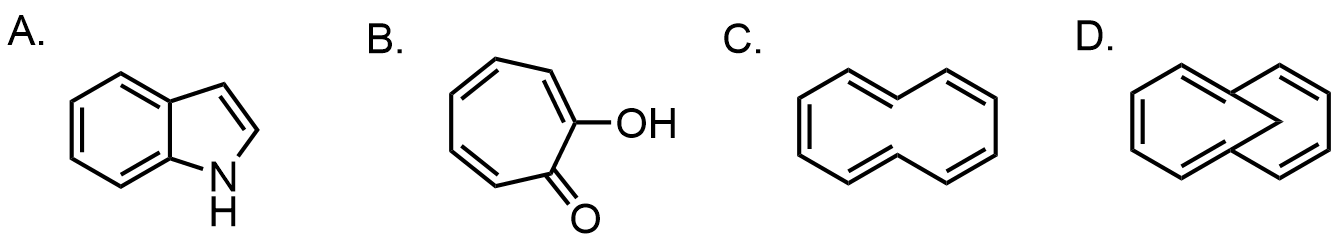
\includegraphics[scale=0.38, valign=c]{./Figure/2015/2015_4_1.png} 
    \item 下列化合物酸性最强的是
    
    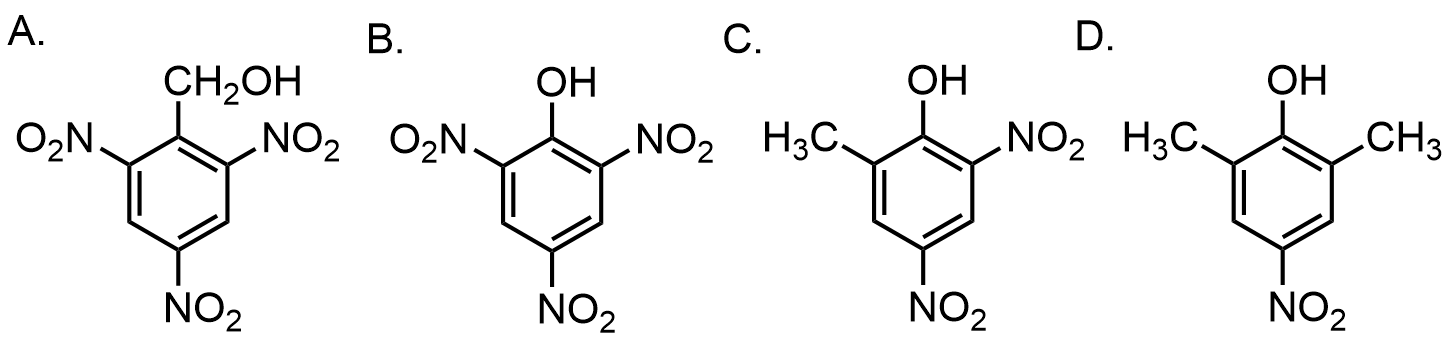
\includegraphics[scale=0.38, valign=c]{./Figure/2015/2015_4_2.png}
    \item 所给出的化合物中手性碳原子的绝对构型是
    
    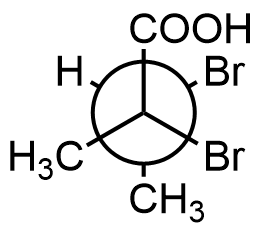
\includegraphics[scale=0.38, valign=c]{./Figure/2015/2015_4_3.png}
    \begin{tasks}(4)
        \task 2R,3R
        \task 2R,3S
        \task 2S,3R
        \task 2S,3S
    \end{tasks}
    \item 下列化合物具有手性的是
    
    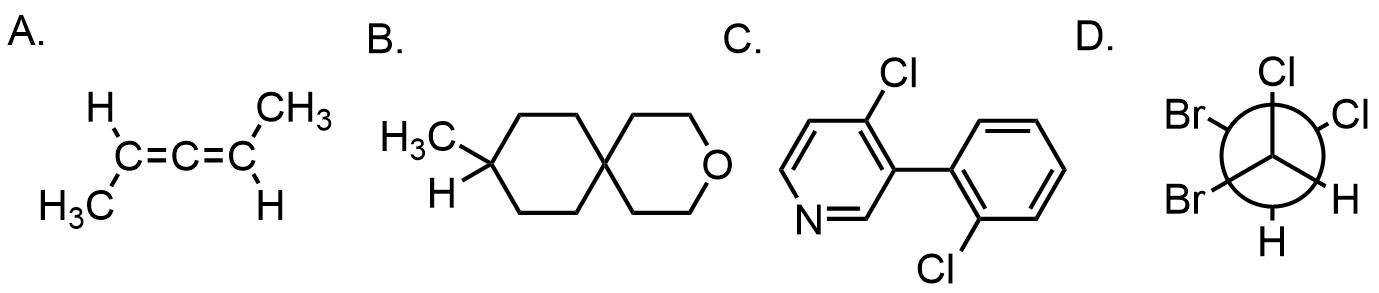
\includegraphics[scale=0.38, valign=c]{./Figure/2015/2015_4_4.png} 
    \item 下列化合物中烯醇式含量最高的是
    \begin{tasks}(2)
        \task \ce{CH3COCH2COCH3}
        \task \ce{CH3COCH2COOCH3}
        \task \ce{CH3COCH2CONH2}
        \task \ce{CH3COCH2CHO}
    \end{tasks}
    \item 可除去苯中少量噻吩的方法是
    \begin{tasks}(2)
        \task 用\ce{NaOH}水溶液洗涤
        \task 用石油醚洗涤
        \task 用\ce{NaHSO3}水溶液洗涤
        \task 用浓硫酸洗涤
    \end{tasks}
    \item 下列溶剂分子中极性最大的是
    \begin{tasks}(4)
        \task \ce{CH3OH}
        \task \ce{C2H5OC2H5}
        \task \ce{ClCH2CH2Cl}
        \task \ce{CHCl3}
    \end{tasks}
    \item 下列化合物中亲核性最强的是
    \begin{tasks}(4)
        \task \ce{CH3CH2SH}
        \task \ce{CH3CH2SNa}
        \task \ce{CH3CH2OH}
        \task \ce{CH3CH2ONa}
    \end{tasks}
    \item 下列化合物中能发生碘仿反应的是
    
    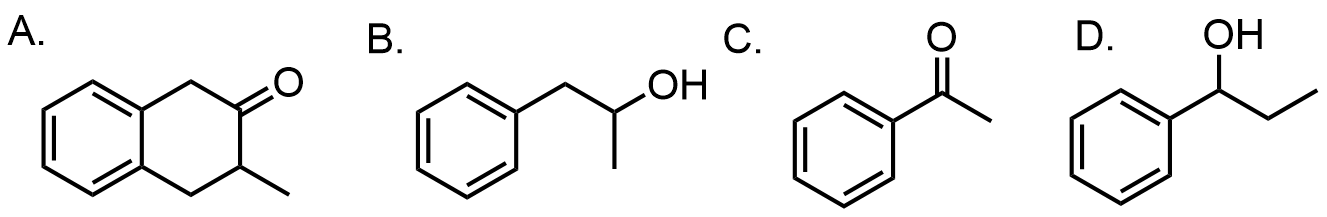
\includegraphics[scale=0.38, valign=c]{./Figure/2015/2015_4_9.png}
    \item 下列化合物与\ce{AgNO3}水溶液反应立刻生成沉淀的是
    
    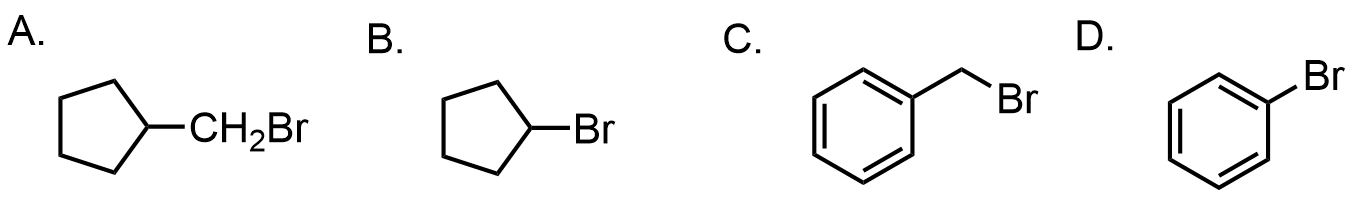
\includegraphics[scale=0.38, valign=c]{./Figure/2015/2015_4_10.png}
    \item 下列自由基中最稳定的是
    
    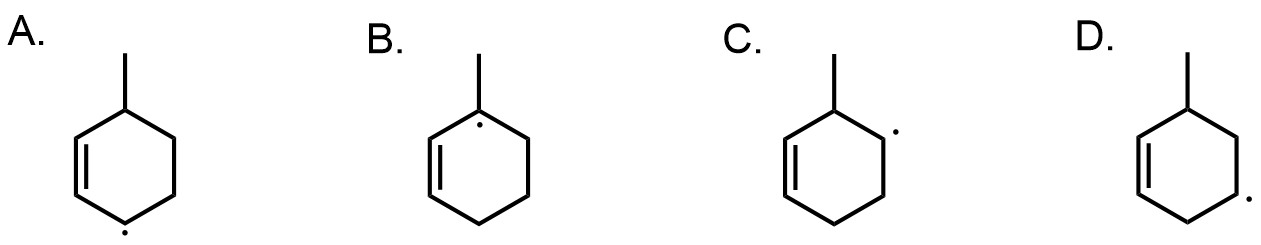
\includegraphics[scale=0.38, valign=c]{./Figure/2015/2015_4_11.png}
    \item 下列化合物与四氢吡咯反应最快的是
    
    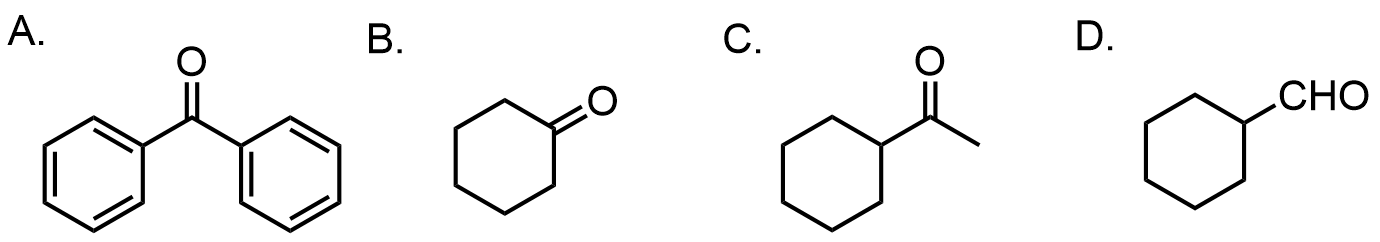
\includegraphics[scale=0.38, valign=c]{./Figure/2015/2015_4_12.png}
    \item 下列基团再芳香亲电取代中具有钝化的邻对位定位作用的是
    \begin{tasks}(4)
        \task \ce{CH3}
        \task \ce{COOH}
        \task \ce{OH}
        \task \ce{Cl}
    \end{tasks}
    \item 下列化合物在碱性条件下水解反应速度最快的是
    \begin{tasks}(2)
        \task \ce{CF3COOC2H5}
        \task \ce{CH3COOC2H5}
        \task \ce{CH3CH2COOC2H5}
        \task \ce{ClCH2COOC2H5}
    \end{tasks}
\end{enumerate}

\vspace{0.5cm}
\noindent\textbf{二、完成反应(40 pts.)}

\begin{enumerate}[label=\arabic*., itemsep=3ex]
    \item 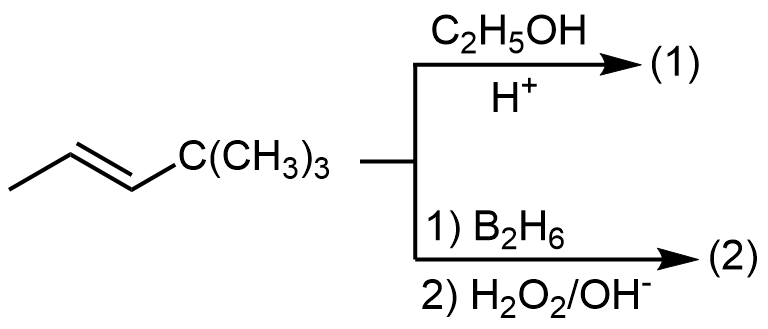
\includegraphics[scale=0.38, valign=c]{./Figure/2015/2015_1_1.png} 
    \item 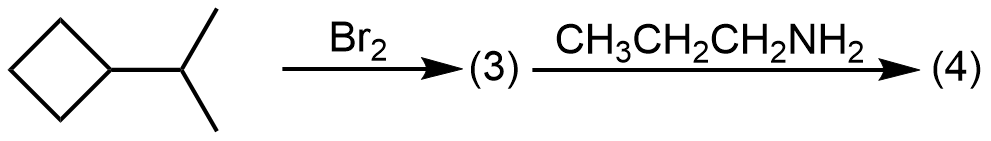
\includegraphics[scale=0.38, valign=c]{./Figure/2015/2015_1_2.png}
    \item 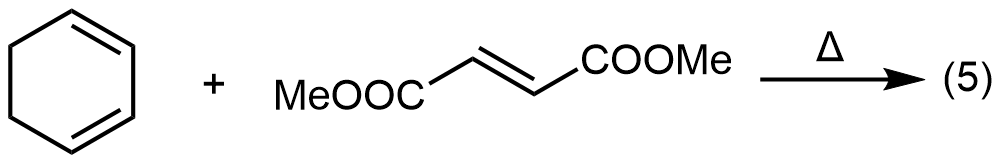
\includegraphics[scale=0.38, valign=c]{./Figure/2015/2015_1_3.png}
    \item 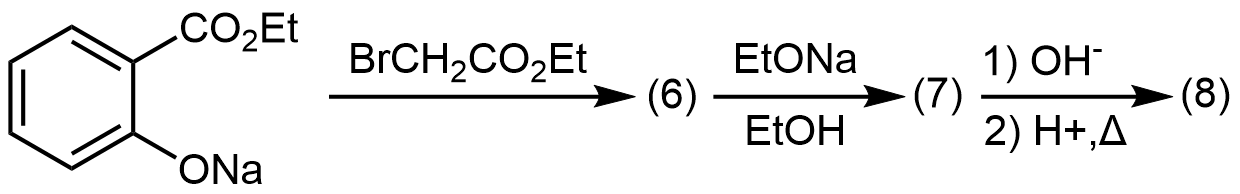
\includegraphics[scale=0.38, valign=c]{./Figure/2015/2015_1_4.png}
    \item 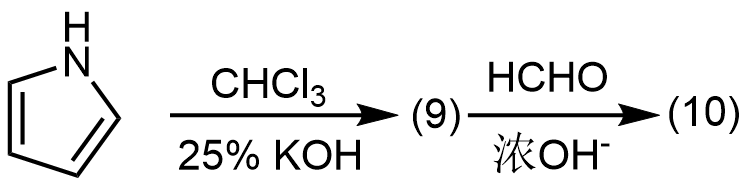
\includegraphics[scale=0.38, valign=c]{./Figure/2015/2015_1_5.png}
    \item 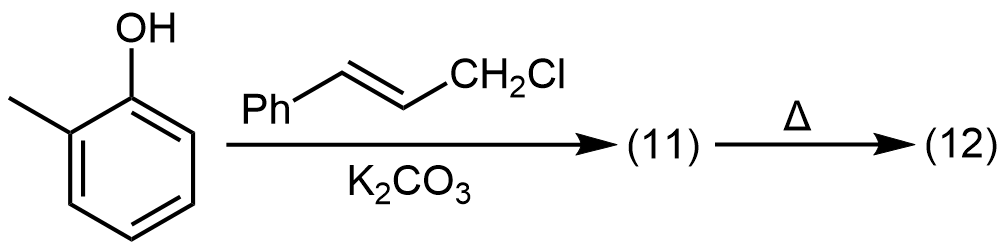
\includegraphics[scale=0.38, valign=c]{./Figure/2015/2015_1_6.png}
    \item 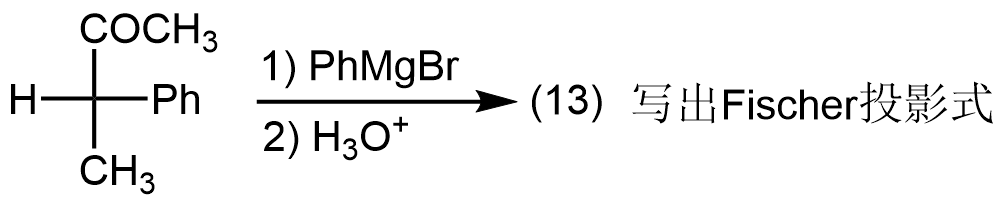
\includegraphics[scale=0.38, valign=c]{./Figure/2015/2015_1_7.png}
    \item 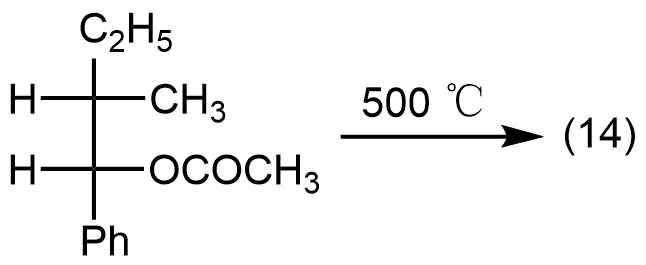
\includegraphics[scale=0.38, valign=c]{./Figure/2015/2015_1_8.png}
    \item 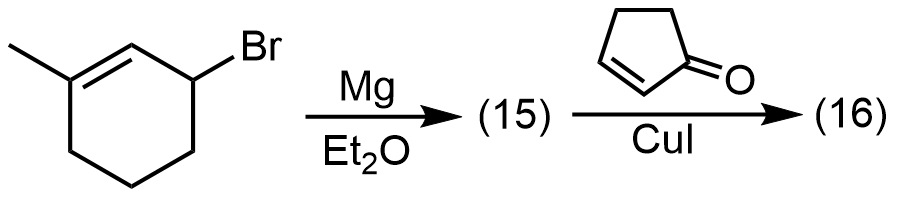
\includegraphics[scale=0.38, valign=c]{./Figure/2015/2015_1_9.png}
    \item 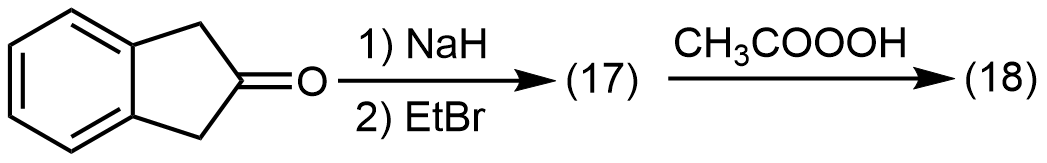
\includegraphics[scale=0.38, valign=c]{./Figure/2015/2015_1_10.png}
    \item 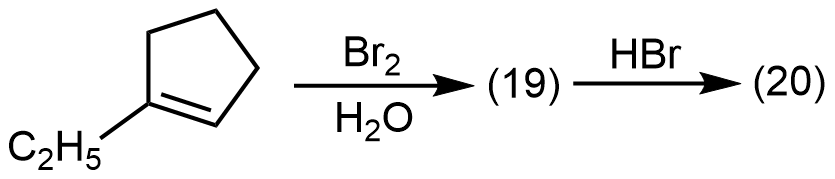
\includegraphics[scale=0.38, valign=c]{./Figure/2015/2015_1_11.png}

\end{enumerate}

\vspace{0.5cm}
\noindent\textbf{三、机理题(32 pts.)}

\begin{enumerate}[label=\arabic*., start=1, itemsep=1.5ex]
    \item 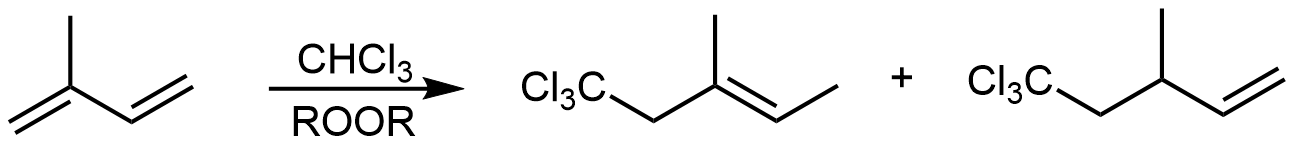
\includegraphics[scale=0.38, valign=c]{./Figure/2015/2015_2_1.png}
    \item 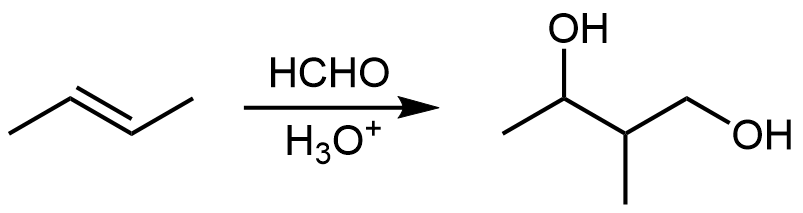
\includegraphics[scale=0.38, valign=c]{./Figure/2015/2015_2_2.png}
    \item 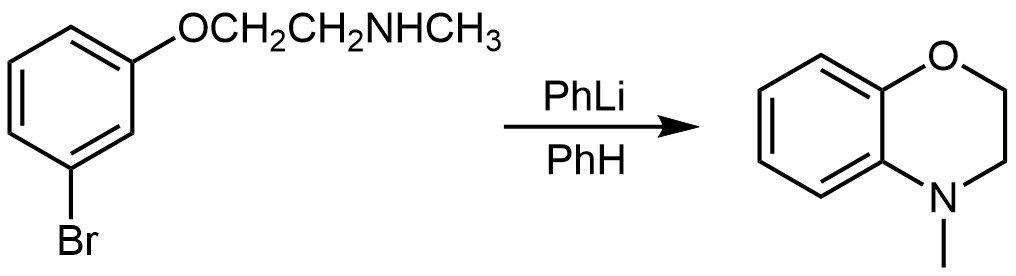
\includegraphics[scale=0.38, valign=c]{./Figure/2015/2015_2_3.png}
    \item 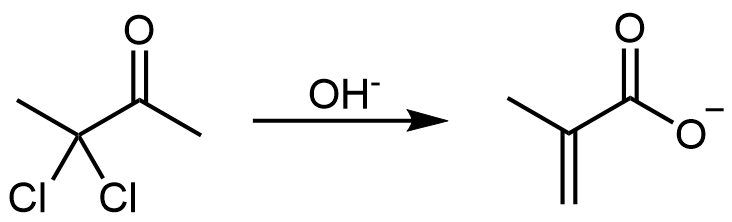
\includegraphics[scale=0.38, valign=c]{./Figure/2015/2015_2_4.png}
\end{enumerate}

\newpage

\vspace{0.5cm}
\noindent\textbf{四、合成题(48 pts.)}

\begin{enumerate}[label=\arabic*., start=1, itemsep=1.5ex]

    \begin{figure}[htbp]
        \centering
        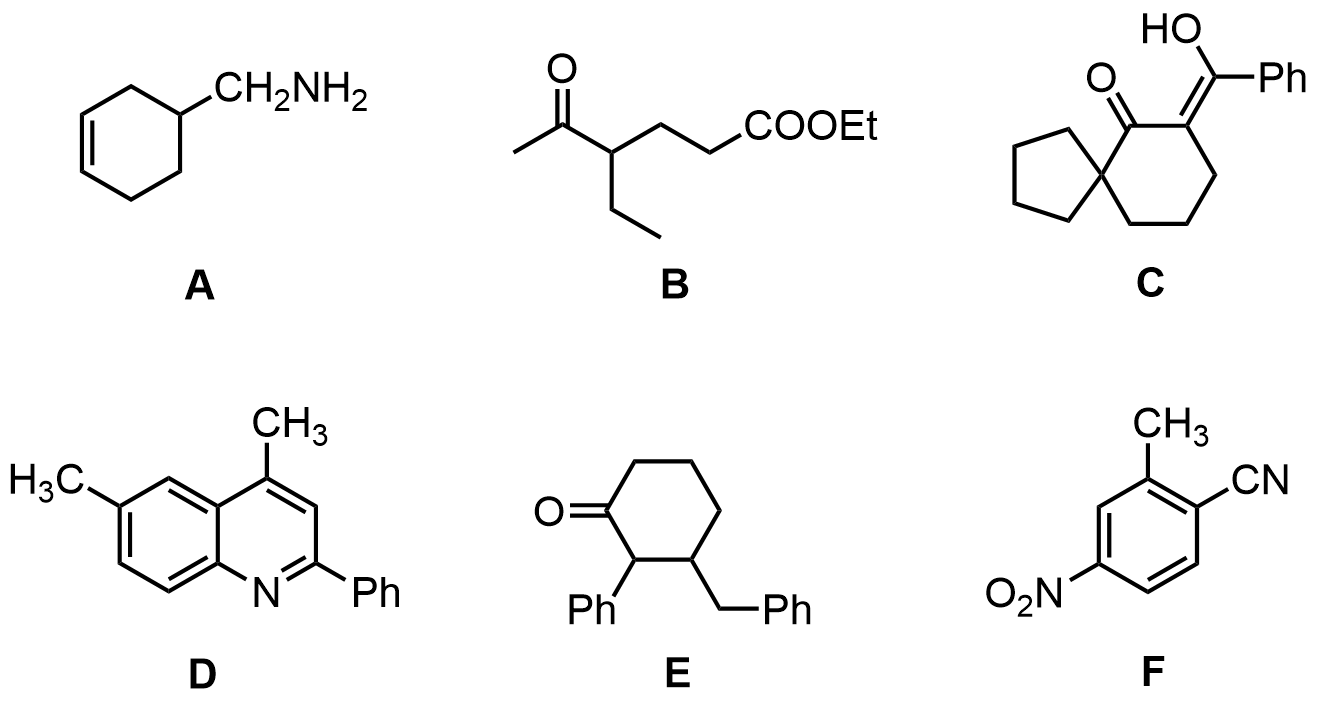
\includegraphics[scale=0.38]{./Figure/2015/2015_3.png}
    \end{figure}
    \item 以乙炔为唯一有机原料合成\textbf{A}
    \item 以乙酰乙酸乙酯、小于等于3个碳的有机物合成\textbf{B}
    \item 以环戊酮和甲苯为唯二有机原料合成\textbf{C}
    \item 以甲苯、小于等于3个碳的有机物合成\textbf{D}
    \item 以环戊烯和苯为唯二有机原料合成\textbf{E}
    \item 以甲苯为唯一有机原料合成\textbf{F}
\end{enumerate}

\vspace{0.5cm}
\noindent\textbf{五、实验题 略}